\scanpage{6}
Utilisant \unsure{th. gr|th. quo}, on aura

\diagram{\begin{tikzcd}[ampersand replacement=\&,row sep=.4em]
T\subset G \arrow[d,phantom,"\rotatebox{-90}{$\supset$}" description] \&[-1em]
{\left\{\begin{aligned}
&T\times H\mathrel{\unsure{-|\longrightarrow}}G\quad\text{imm. ouverte}\\
&\deleted{\unsure{T\cap H=e}}\quad\bigcap\ \text{conjugués de }H=e
\end{aligned}\right.}\\
\hphantom{T\subset{}}H \&
\end{tikzcd}}

On aura pseudomorphisme $\mathrm{pr}_1$
\diagram{\begin{tikzcd}[ampersand replacement=\&] G\arrow[r,dashed,"f"] \& T \end{tikzcd}}
\[
\begin{aligned}
&[\,\text{pseudo-opération est}\qquad (g,t)\mapsto f(gt)\,]\\
&\hspace{13em}\rotatebox{90}{$=$}\\[-2pt]
&\hspace{12em}t f(t^{-1}gt)
\end{aligned}
\]

\uline{Axiomes sur $f$}
\[
\left\{\begin{aligned}
1)\quad &f(gg')=f(gf(g'))\quad \text{(si }f(g')\text{ est défini, les 2 \unsure{mbs|sens} le}\\
&\hspace{16em}\text{sont simultanément)}\\
2)\quad &f\ \text{défini en tt pt de }T,\ \text{et y induit l'identité}\\
3)\quad &\text{Si }g,g'\in G(S),\ \text{et }f(gt)\equiv f(g't)\ \text{pour tt }t\ \ldots-,\\
&\text{alors }g=g'.
\end{aligned}\right.
\]

\[
\Longrightarrow \qquad f(tg)=tf(g)
\]

\figure{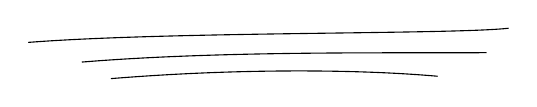
\begin{tikzpicture}[x=1cm,y=1cm]
\draw (0,0) .. controls (1.8,.14) and (5.4,.10) .. (6.1,.18);
\draw (.68,-.25) .. controls (2.5,-.10) and (4.8,-.14) .. (5.82,-.13);
\draw (1.05,-.46) .. controls (2.65,-.33) and (4.18,-.34) .. (5.2,-.43);
\end{tikzpicture}}
% archive sheet number: 5
